%%%%%%%%%%%%%%%%%%%%%%%%%%%%%%%%%%%%%%%%%%%%%%%%%%%%%%%%%%%%%%%%%%%%%%%%%%%%%%%%%%%%%
%%%%%%%%%%%%%%%%%%%%%%%%%%%%%%%%%%%%%%%%%%%%%%%%%%%%%%%%%%%%%%%%%%%%%%%%%%%%%%%%%%%%%

\setbeamercolor{block body}{bg=blue!20}

\begin{frame}
\frametitle{Borealis compilation scheme}
	\begin{figure}
		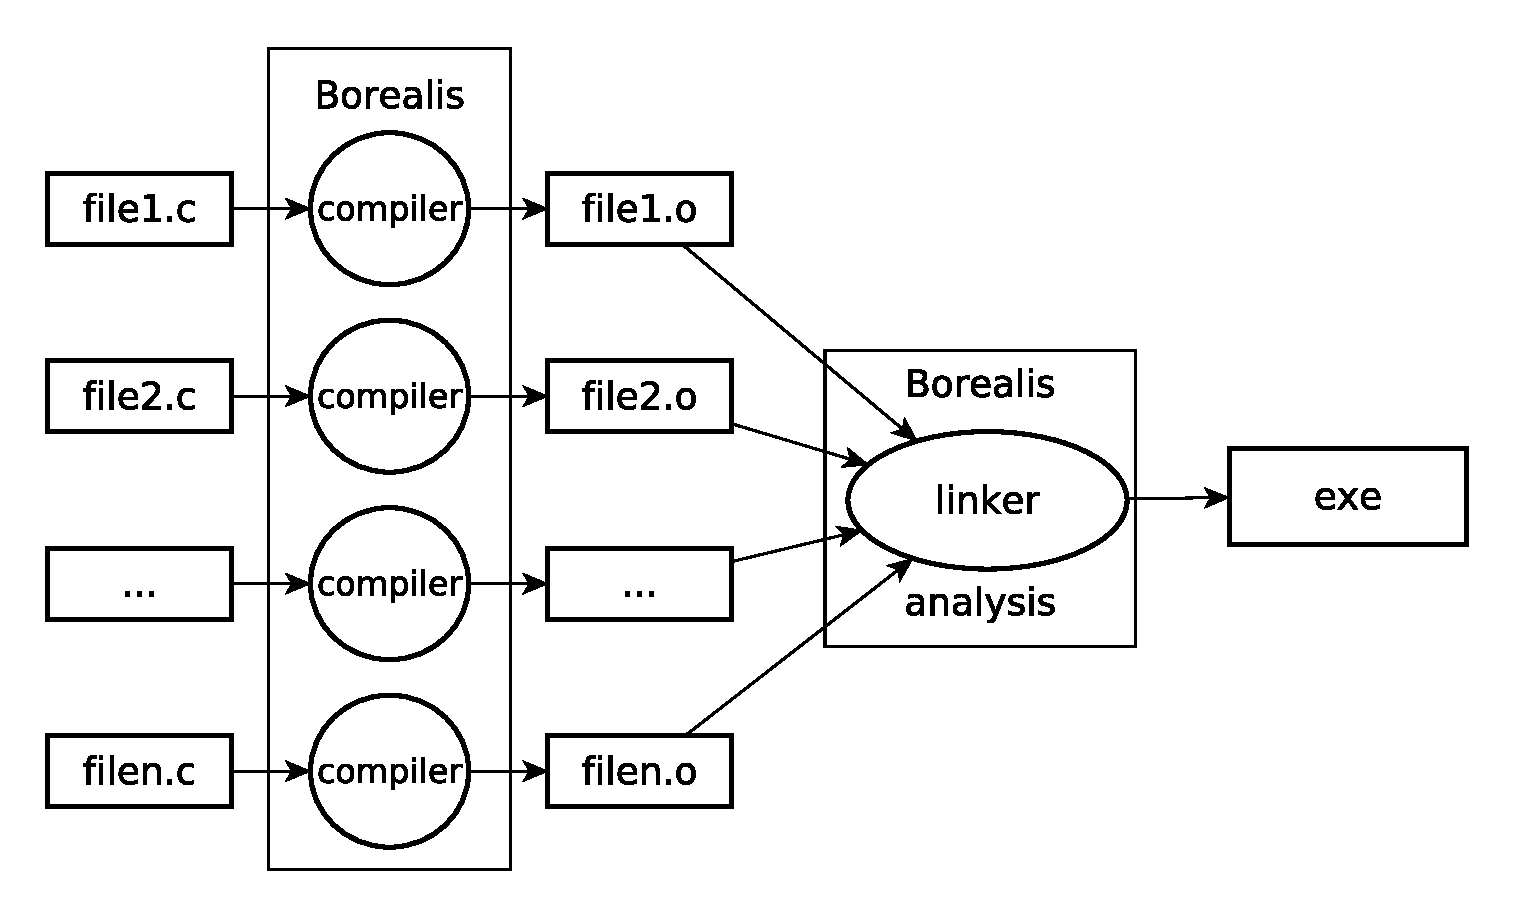
\includegraphics[width=115mm]{image/compile}
	\end{figure}	
\end{frame}


%%%%%%%%%%%%%%%%%%%%%%%%%%%%%%%%%%%%%%%%%%%%%%%%%%%%%%%%%%%%%%%%%%%%%%%%%%%%%%%%%%%%%
%%%%%%%%%%%%%%%%%%%%%%%%%%%%%%%%%%%%%%%%%%%%%%%%%%%%%%%%%%%%%%%%%%%%%%%%%%%%%%%%%%%%%

\begin{frame}
\frametitle{Distributed compilation}
There are several ways to distributed compilation:
\begin{itemize}
	\item Compilation on the Lustre storage
	\item Distribution of intermediate build tree to the processing nodes
	\item Distribution of copies of the analyzed project
\end{itemize} 
\end{frame}

%%%%%%%%%%%%%%%%%%%%%%%%%%%%%%%%%%%%%%%%%%%%%%%%%%%%%%%%%%%%%%%%%%%%%%%%%%%%%%%%%%%%%
%%%%%%%%%%%%%%%%%%%%%%%%%%%%%%%%%%%%%%%%%%%%%%%%%%%%%%%%%%%%%%%%%%%%%%%%%%%%%%%%%%%%%

\begin{frame}
\frametitle{Compilation on the Lustre storage}
\begin{itemize}
\item Each node access to Lustre for necessary files
\item Lustre is slow when dealing with multiple small files
\end{itemize}
	\begin{figure}
		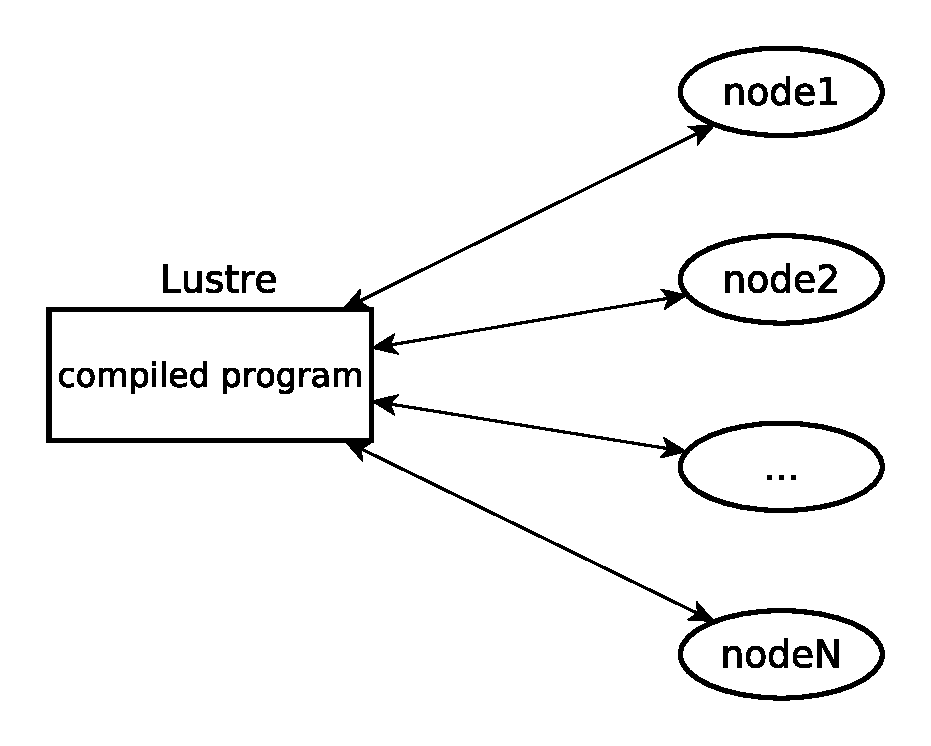
\includegraphics[width=70mm]{image/compLustre}
	\end{figure}	
\end{frame}

%%%%%%%%%%%%%%%%%%%%%%%%%%%%%%%%%%%%%%%%%%%%%%%%%%%%%%%%%%%%%%%%%%%%%%%%%%%%%%%%%%%%%
%%%%%%%%%%%%%%%%%%%%%%%%%%%%%%%%%%%%%%%%%%%%%%%%%%%%%%%%%%%%%%%%%%%%%%%%%%%%%%%%%%%%%

\begin{frame}
\frametitle{Distribution of intermediate build tree}
\begin{itemize}
\item Reduce the CPU time
\item Build may contain several related compilation/linking phases
\end{itemize}
	\begin{figure}
		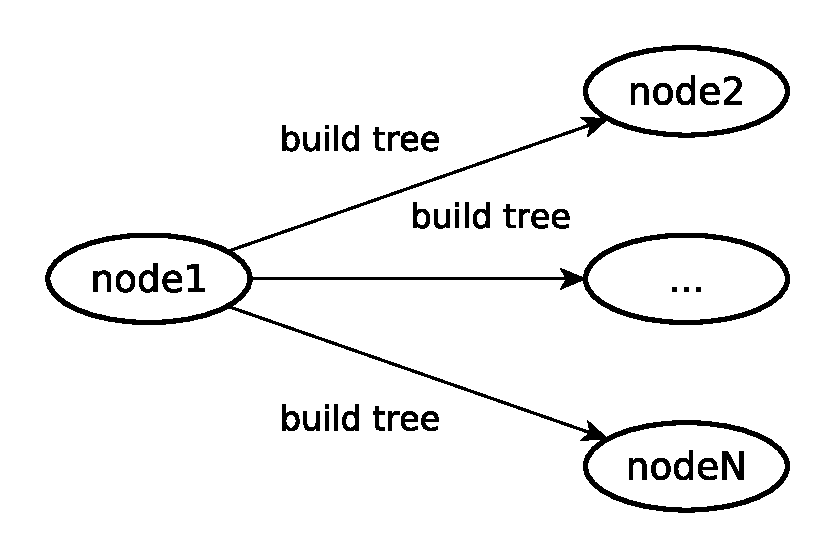
\includegraphics[width=70mm]{image/compTree}
	\end{figure}	
\end{frame}

%%%%%%%%%%%%%%%%%%%%%%%%%%%%%%%%%%%%%%%%%%%%%%%%%%%%%%%%%%%%%%%%%%%%%%%%%%%%%%%%%%%%%
%%%%%%%%%%%%%%%%%%%%%%%%%%%%%%%%%%%%%%%%%%%%%%%%%%%%%%%%%%%%%%%%%%%%%%%%%%%%%%%%%%%%%

\begin{frame}
\frametitle{Distribution of copies of the analyzed project}
\begin{itemize}
\item Compilation is done using standard build tools
\item We are repeating computations on every node
\item Don't increase the wall-clock time
\end{itemize}
	\begin{figure}
		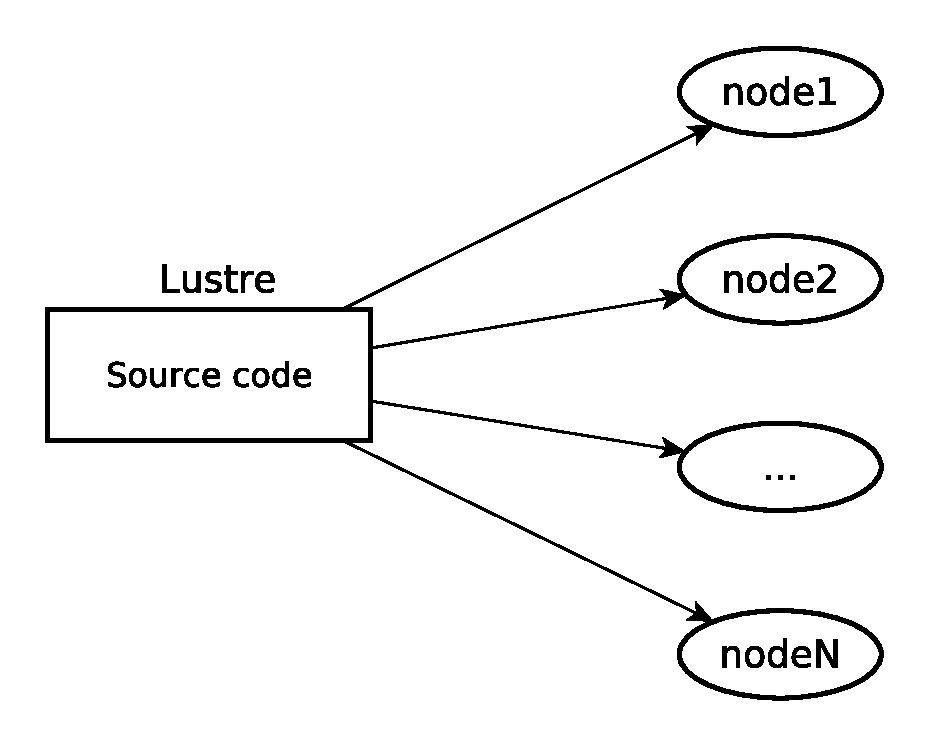
\includegraphics[width=110mm]{image/compSource}
	\end{figure}	
\end{frame}

%%%%%%%%%%%%%%%%%%%%%%%%%%%%%%%%%%%%%%%%%%%%%%%%%%%%%%%%%%%%%%%%%%%%%%%%%%%%%%%%%%%%%
%%%%%%%%%%%%%%%%%%%%%%%%%%%%%%%%%%%%%%%%%%%%%%%%%%%%%%%%%%%%%%%%%%%%%%%%%%%%%%%%%%%%%
\begin{frame}
\frametitle{Distributed linking}
\begin{itemize}
	\item We distribute different SMT queries to different nodes/cores 
	\item Borealis performs analysis on an LLVM IR module
\end{itemize}
\end{frame}

%%%%%%%%%%%%%%%%%%%%%%%%%%%%%%%%%%%%%%%%%%%%%%%%%%%%%%%%%%%%%%%%%%%%%%%%%%%%%%%%%%%%%
%%%%%%%%%%%%%%%%%%%%%%%%%%%%%%%%%%%%%%%%%%%%%%%%%%%%%%%%%%%%%%%%%%%%%%%%%%%%%%%%%%%%%
\begin{frame}
\frametitle{Distributed linking}
It means there are options of how one can distribute the work:
\begin{itemize}
	\item Module level
	\begin{itemize}
	    \item[•] Same as parallel make
	    \item[•] Not really effective
	\end{itemize}
	\item Instruction level
		\begin{itemize}
	        \item[•] Need to track dependencies between SMT calls
	        \item[•] Too complex
		\end{itemize}
	\item Function level
	    \begin{itemize}
	        \item[•] Medium efficiency
	        \item[•] Simple implementation
	    \end{itemize}
\end{itemize}
\end{frame}
%%%%%%%%%%%%%%%%%%%%%%%%%%%%%%%%%%%%%%%%%%%%%%%%%%%%%%%%%%%%%%%%%%%%%%%%%%%%%%%%%%%%%
%%%%%%%%%%%%%%%%%%%%%%%%%%%%%%%%%%%%%%%%%%%%%%%%%%%%%%%%%%%%%%%%%%%%%%%%%%%%%%%%%%%%%

\begin{frame}
\frametitle{Distributed linking}
There are two ways how one can distribute functions between several processes:
	\begin{itemize}
		\item Dynamic distribution
		\item Static distribution
	\end{itemize}
\end{frame}

%%%%%%%%%%%%%%%%%%%%%%%%%%%%%%%%%%%%%%%%%%%%%%%%%%%%%%%%%%%%%%%%%%%%%%%%%%%%%%%%%%%%%
%%%%%%%%%%%%%%%%%%%%%%%%%%%%%%%%%%%%%%%%%%%%%%%%%%%%%%%%%%%%%%%%%%%%%%%%%%%%%%%%%%%%%

\begin{frame}
\frametitle{Dynamic distribution}
\begin{itemize}
\item Master process distributes functions between several processes
\item Based on a single producer / multiple consumers scheme
\item If a process receives N functions, it also has to run auxiliary LLVM passes N times
\end{itemize}
	\begin{figure}
		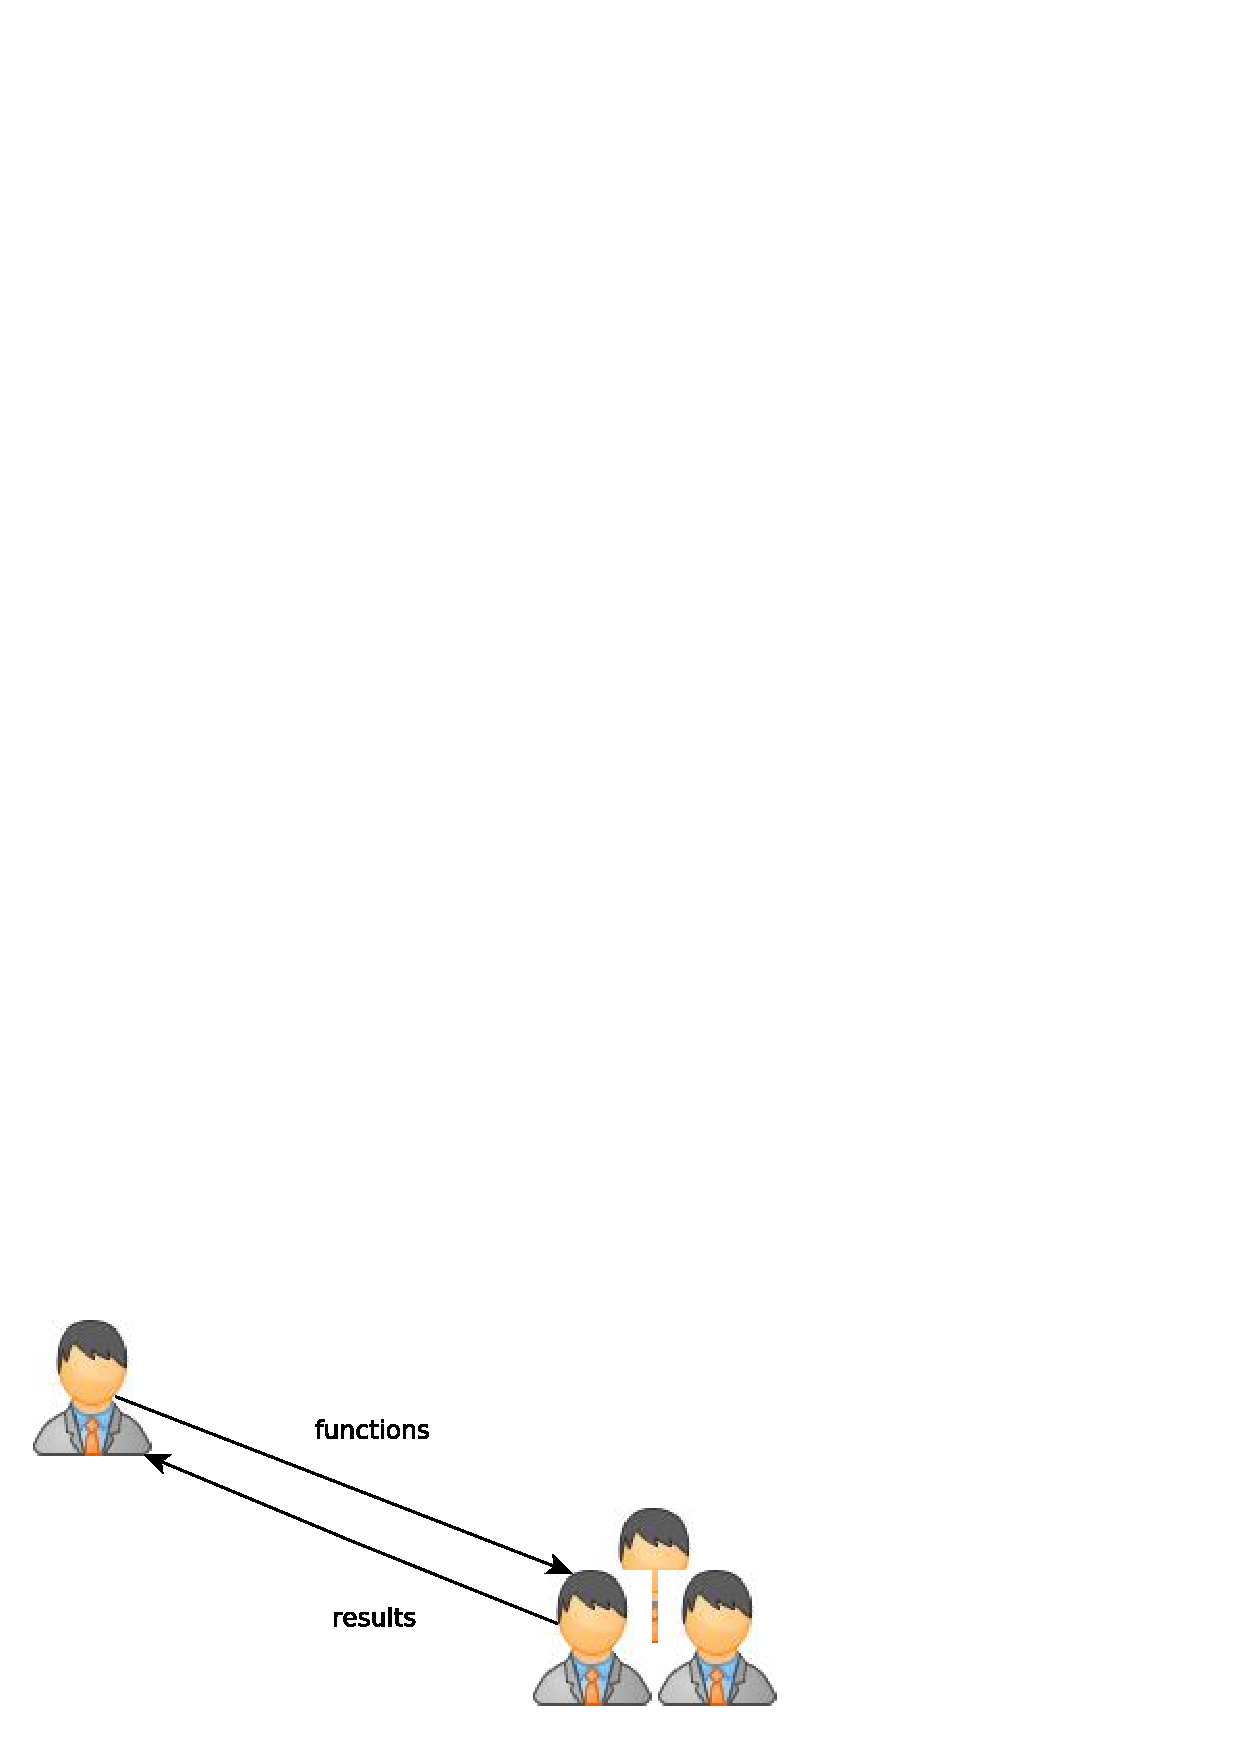
\includegraphics[width=70mm]{image/dynDistr.png}
	\end{figure}	
\end{frame}

%%%%%%%%%%%%%%%%%%%%%%%%%%%%%%%%%%%%%%%%%%%%%%%%%%%%%%%%%%%%%%%%%%%%%%%%%%%%%%%%%%%%%
%%%%%%%%%%%%%%%%%%%%%%%%%%%%%%%%%%%%%%%%%%%%%%%%%%%%%%%%%%%%%%%%%%%%%%%%%%%%%%%%%%%%%

\begin{frame}
\frametitle{Static distribution}
\begin{itemize}
\item Each process determines a set of function based on it's rank
\item We use the following two rank kinds:
	\begin{itemize}
		\item[•] global rank
		\item[•] local rank 
	\end{itemize}
\item After some experiments we decided to use static distribution
\end{itemize}
	\begin{figure}
		\includegraphics[width=70mm]{image/statDistr.png}
	\end{figure}	
\end{frame}

%%%%%%%%%%%%%%%%%%%%%%%%%%%%%%%%%%%%%%%%%%%%%%%%%%%%%%%%%%%%%%%%%%%%%%%%%%%%%%%%%%%%%
%%%%%%%%%%%%%%%%%%%%%%%%%%%%%%%%%%%%%%%%%%%%%%%%%%%%%%%%%%%%%%%%%%%%%%%%%%%%%%%%%%%%%

\begin{frame}
\frametitle{Improving static distribution}
\begin{itemize}
\item Need to balance workload
\item We reinforce method with function complexity estimation
\item Our estimation is based on the following properties:
	\begin{itemize}
		\item[•] Function size
		\item[•] Number of memory work instructions
	\end{itemize}
\end{itemize}
\end{frame}

%%%%%%%%%%%%%%%%%%%%%%%%%%%%%%%%%%%%%%%%%%%%%%%%%%%%%%%%%%%%%%%%%%%%%%%%%%%%%%%%%%%%%
%%%%%%%%%%%%%%%%%%%%%%%%%%%%%%%%%%%%%%%%%%%%%%%%%%%%%%%%%%%%%%%%%%%%%%%%%%%%%%%%%%%%%

\begin{frame}[fragile]
\frametitle{PDD}
\begin{itemize}
\item Borealis records the analysis results  
\item Thereby we doesn't re-analyze already processed functions
\item Persistent Defect Data (PDD) is used for recording results
\item PDD contains:
	\begin{itemize}
		\item[•] Defect location
		\item[•] Defect type
		\item[•] SMT result
	\end{itemize}
\end{itemize}
\begin{columns} 
\column{0.5\textwidth} 
\begin{lstlisting}[style=crs_cpp] 
{
    "location": {
        "loc": {
            "col": 2,
            "line": 383
        },
        "filename": "rarpd.c"
    },
    "type": "INI-03"
}
\end{lstlisting} 
\end{columns}
\end{frame}

%%%%%%%%%%%%%%%%%%%%%%%%%%%%%%%%%%%%%%%%%%%%%%%%%%%%%%%%%%%%%%%%%%%%%%%%%%%%%%%%%%%%%
%%%%%%%%%%%%%%%%%%%%%%%%%%%%%%%%%%%%%%%%%%%%%%%%%%%%%%%%%%%%%%%%%%%%%%%%%%%%%%%%%%%%%

\begin{frame}[fragile]
\frametitle{PDD synchronization problem}
\begin{itemize}
\item Transfer a full PDD takes a long time
\item We synchronize a reduced PDD (rPDD)
\item rPDD is simply a list of already analyzed functions
\end{itemize}
\end{frame}

%%%%%%%%%%%%%%%%%%%%%%%%%%%%%%%%%%%%%%%%%%%%%%%%%%%%%%%%%%%%%%%%%%%%%%%%%%%%%%%%%%%%%
%%%%%%%%%%%%%%%%%%%%%%%%%%%%%%%%%%%%%%%%%%%%%%%%%%%%%%%%%%%%%%%%%%%%%%%%%%%%%%%%%%%%%

\begin{frame}
\frametitle{rPDD synchronization}
To make the synchronization we utilize a two-staged approach:
	\begin{itemize}
		\item Synchronize rPDD between the processes on a single node
		\item Synchronize rPDD between the nodes
\end{itemize}
	\begin{figure}
		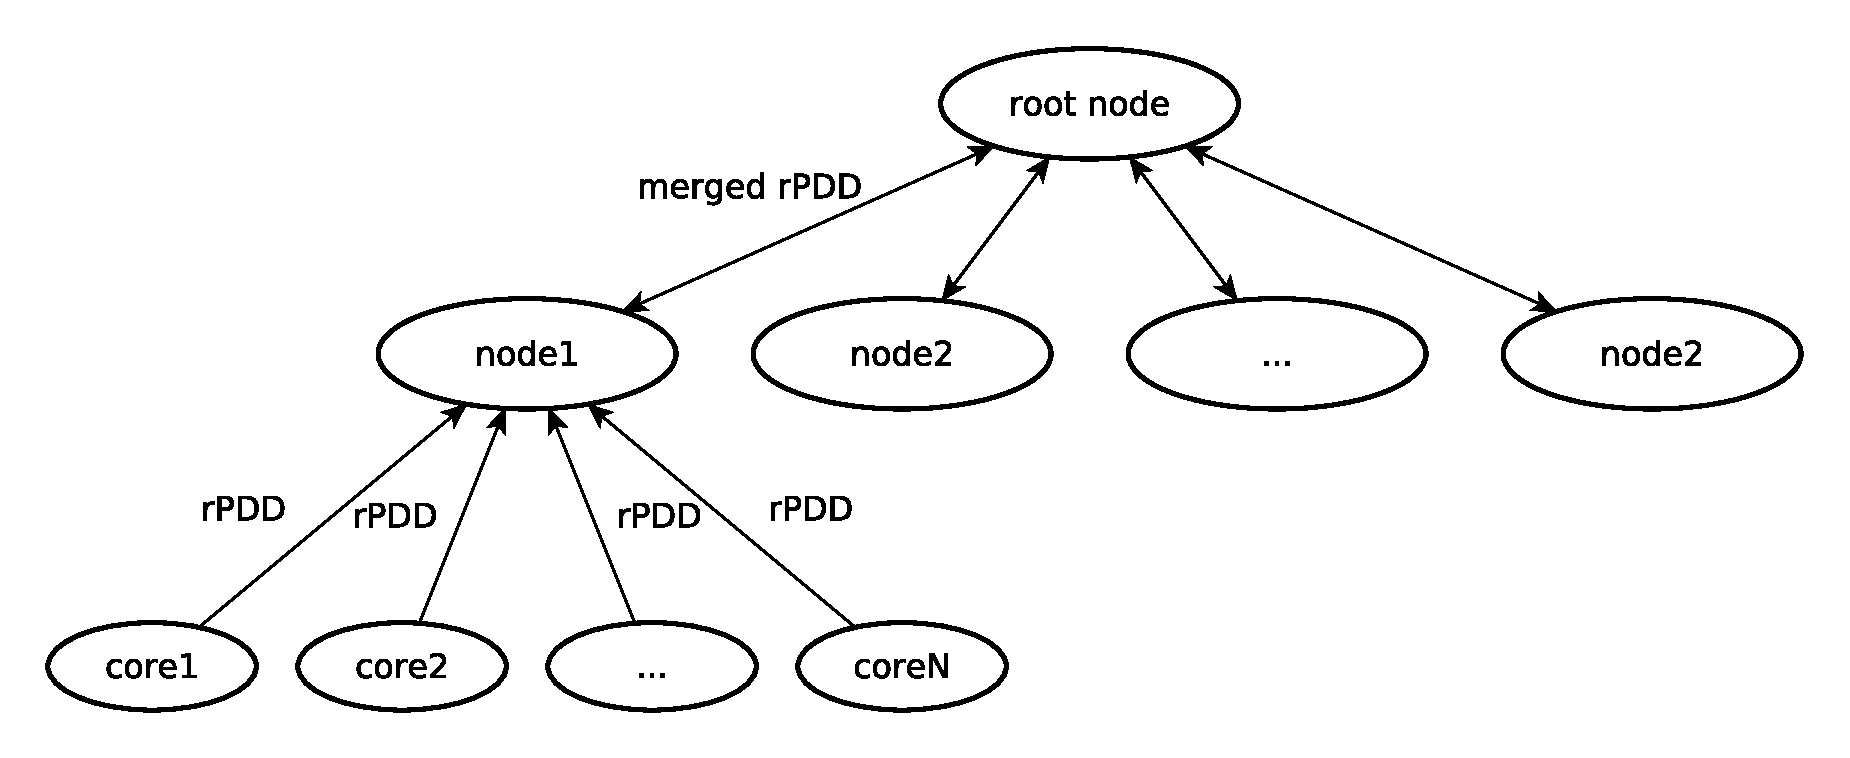
\includegraphics[width=115mm]{image/pddMerge}
	\end{figure}	
\end{frame}

%%%%%%%%%%%%%%%%%%%%%%%%%%%%%%%%%%%%%%%%%%%%%%%%%%%%%%%%%%%%%%%%%%%%%%%%%%%%%%%%%%%%%
%%%%%%%%%%%%%%%%%%%%%%%%%%%%%%%%%%%%%%%%%%%%%%%%%%%%%%%%%%%%%%%%%%%%%%%%%%%%%%%%%%%%%

\begin{frame}
\frametitle{Implementation}
\begin{itemize}
	\item Borealis HPC implementation is based on OpenMPI library
	\item We implemented API to work with library
	\item HPC Borealis is implemented in the form of 3 LLVM passes
\end{itemize}
	\begin{figure}
		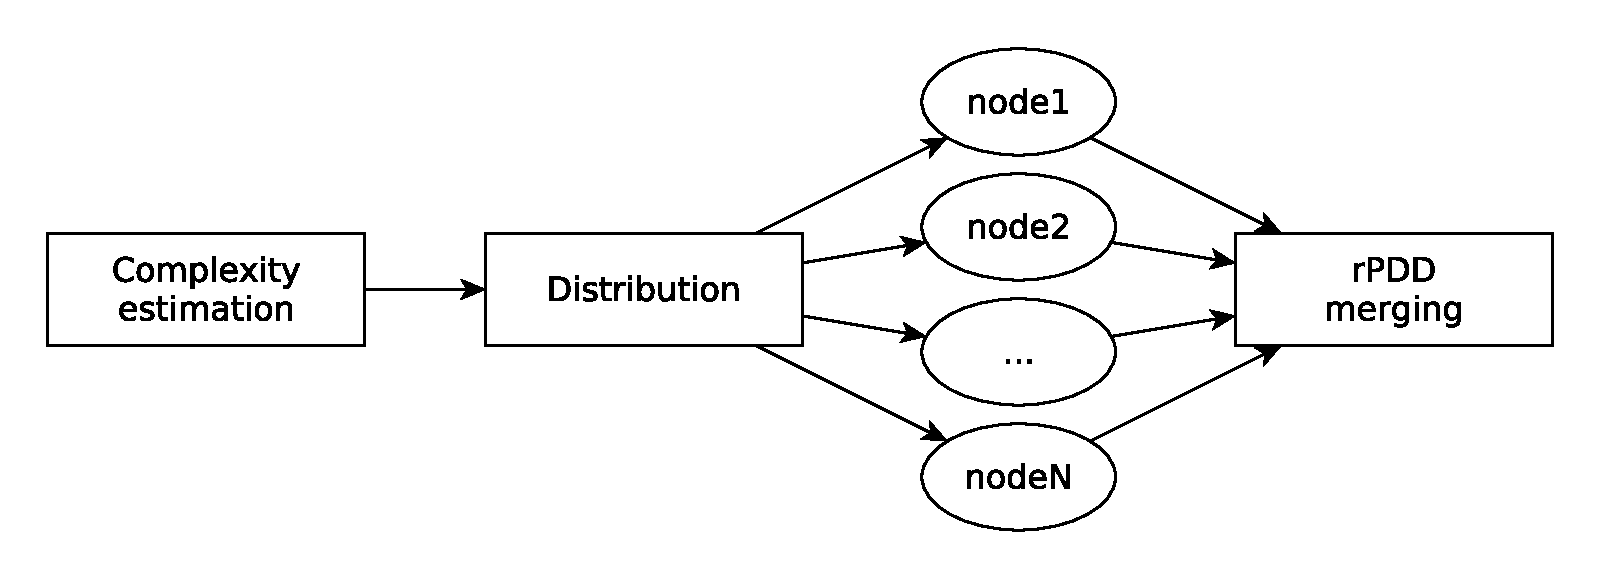
\includegraphics[width=100mm]{image/passes}
	\end{figure}	
\end{frame}
%%%%%%%%%%%%%%%%%%%%%%%%%%%%%%%%%%%%%%%%%%%%%%%%%%%%%%%%%%%%%%%%%%%%%%%%%%%%%%%%%%%%%
%%%%%%%%%%%%%%%%%%%%%%%%%%%%%%%%%%%%%%%%%%%%%%%%%%%%%%%%%%%%%%%%%%%%%%%%%%%%%%%%%%%%%

